\chapter{Theory}


\section{Machine Learning}
Machine learning, or ML for short, is a branch of artificial intelligence (AI) that focuses on creating computer algorithms that learn automatically from data and experience. It allows computers to learn from data and make predictions or decisions without the need for explicit programming.
With the rapid advancement of AI, machines are now able to solve complex problems with greater ease. Learning methods can be broadly classified into two main categories - supervised learning and unsupervised learning. In addition to these, there are other methods such as reinforcement learning, semi-supervised learning, and many hybrid approaches.

Supervised learning involves training a computer algorithm with input data that has been labeled for a specific output. To enable it to produce accurate labeling results when presented with never-before-seen data, the model is trained until it can identify the underlying patterns and relationships between the input data and the output labels. Making sense of the data for a particular question is the goal of supervised learning. Classification and regression problems are well-suited for supervised learning. 


With classification, one of a known number of categories is represented by the output variable. For instance, "dog" or "cat," "positive" or "negative." Popular techniques used for classification involve a logistic regression, a decision tree, a random forest, or a support vector machine.


The regression's value of the output variable is continuous or actual. For instance, "geographical location", and "price". The following algorithms are frequently employed: linear regression, nonlinear regression, a regression tree, or Bayesian logic.


Unsupervised learning relies on an unlabeled dataset for training, without requiring any correct output values as in supervised learning. Instead, the algorithm identifies patterns and similarities within the data, independent of external measurements. This approach allows algorithms to explore and uncover unexpected insights that may not have been anticipated by humans.

Two more problem categories for the unsupervised learning algorithm are clustering and association.


With clustering, objects are grouped into clusters, so that those with the greatest similarities stay in that group and have little to no similarities with other objects in the group.


An association rule is used to determine the relationships between variables in a large database. An association rule improves the efficacy of marketing strategy. For example, consumers who purchase X (bread, for example) also frequently buy Y (butter).


Some of the popular unsupervised learning algorithms include K-means clustering, KNN, hierarchal clustering, or anomaly detection.

\section{Techniques used in Computer Vision }
In Computer Vision (CV), ML plays an important role in extracting important information from images. CV successfully contributes to various domains, surveillance systems, optical character recognition, robotics, suspect detection, and many more.  The direction of CV research is going towards the healthcare domain, medical imaging (MI) is an emerging technology, that plays a vital role in improving image quality and recognizing critical features of binary medical images, covert original images into grayscale, and set the threshold for segmentation.
Within computer vision, three key tasks stand out: segmentation, detection, and classification.
\subsection*{Image Classifiaction}
It's a known fact that the image we see as a whole is made up of hundreds to thousands of tiny pixels. Before computer vision can determine and label the image as a whole, it needs to analyze the individual components of the image. That is why image classification techniques analyze a given image in the form of pixels and accomplish this by treating the picture as an array of matrices, the size of which is determined by the image resolution. The pixels of the digital image are taken and grouped into what we know as “classes.” From this point on, the procedure will vary depending on the algorithm. To guarantee that it is not left entirely on the final classifier, the selected algorithm will convert the image into a series of key attributes. These characteristics aid the classifier in identifying the subject matter and class to which the image belongs.
We can say that the image classification pipeline looks like this:
image pre-processing -> feature extraction -> object classification


Based on the nature of the problem, there are different types of image classification methodologies. They are binary, multiclass, multilabel, and hierarchical.

Binary classification divides unknown data points into two groups using an either-or logic for labeling images. Binary classification is used to handle many different yes/no problems, such as analyzing product quality to determine whether a product has faults, and many more tasks requiring judgment calls.

As the name implies, multiclass divides objects into three or more classes, whereas binary classification divides objects into two classes. It's highly helpful in a variety of fields, including medical diagnostics (disease categorization), NLP (sentiment analysis in situations involving several emotions), etc.

The multilabel method permits an object to be allocated to more than one label, in contrast to multiclass classification, which assigns an image to a single class. For instance, you could have to categorize multiple colors in an image. Taking a picture of a salad, a picture of one will feature red, orange, yellow, purple, and other colors. Consequently, several colors will be used as labels on a single image.

The process of classifying classes into a hierarchical structure based on their similarities is known as hierarchical classification. A lower-level class is more definite and detailed, while a higher-level class represents larger categories. If we're classifying a dog, our first model would recognize a dog vs another animal. If a dog is correctly predicted, another model will be used to classify the breed of the dog into border collie, golden retriever, and poodle. All features of higher-class attributes will be hierarchically contained in the latter ones. Hierarchy allows for effective information transfer between related classes as well as a flexible and interpretable framework for organizing and representing complex visual concepts.


Image Classification correlates one class from the training data with a whole image or video frame regardless of the amount of information present. It involves assigning labels and is suitable when fine-grained information is not necessary. During the model training stage, publically accessible datasets are frequently employed to enable correct data labeling.
\subsection*{Object Detection}
The classification is advanced in object detection. It not only classifies many objects in an image but also provides annotations for the bounding boxes that correspond to each entity's position. The CV model's extra benefits enable its implementation in several practical contexts as these models are only a small portion of detecting, labeling, and annotating objects in images or videos. Faster R-CNN \cite{girshick2014rich}, YOLO (You Only Look Once) \cite{redmon2016you}, and SSD (Single Shot MultiBox Detector)\cite{liu2016ssd} are a few popular object detection algorithms. These algorithms are tailored to specific application requirements and differ in terms of speed, accuracy, and trade-offs.  An example of an object detection model is a model for human detection. The model would return a bounding box around each person with a label

\begin{figure}[ht]
	\centering
	\begin{minipage}{0.4\textwidth}
		\centering
		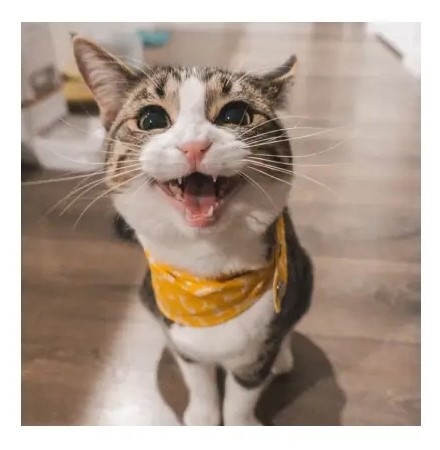
\includegraphics[width=0.7\linewidth]{images/cat_class.jpg}
		\caption*{Cat}
		\label{fig:justcat}
	\end{minipage}% <-- Add this percentage sign here
	\begin{minipage}{0.48\textwidth}
		\centering
		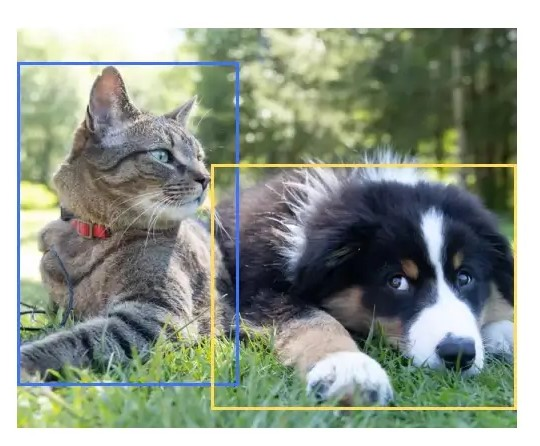
\includegraphics[width=0.7\linewidth]{images/catanddog_detect.jpg}
		\caption*{Cat, Dog}
		\label{fig:catanddog}
	\end{minipage}
	\caption{Comparison of classification (left) with output: 'Cat' and object detection (right) with output: 'Cat, Dog' and their localization with bounding boxes }
	\label{fig:both_figures_class_detect} % This label can now be used to reference both images together
\end{figure}



\subsection*{Image Segmentation}

Since they both serve the same purpose, object detection and image segmentation are comparable. Both techniques identify items in pictures and provide coordinates for locating objects. However, segmentation algorithms produce accurate masks that cover objects at the pixel level, as opposed to creating whole boxes around them.

Annotations for image segmentation include the exact pixel locations of any instances that are present in the image. Image segmentation is better suitable for practical uses because of its accurate results. However, compared to object detection, picture segmentation models are computationally expensive due to algorithm complexity.
The example used is in applying visual effects like background blurring and makeup effects to the image. The functionality identifies specific textures, colors, and segments of object features within image data. It is also widely used in medical imaging, self-driving cars, or satellite imaging.

In figure \ref{fig:segmentation} a U-Net \cite{ronneberger2015u}, an architecture introduced by Olaf Ronneberger, Philipp Fischer, and Thomas Brox in 2015 is used. It's a convolutional neural network that was specifically designed to be used in Biomedical Imaging. A pre-trained model MobileNetV2 \cite{sandler2018mobilenetv2} is used as a lightweight, efficient feature extractor for the input image. It would analyze the photo of the dog and create a set of feature maps highlighting important visual attributes like edges, textures, and shapes relevant to the segmentation task. Then, with the feature maps provided by MobileNetV2, U-Net would take on the task of image segmentation. Its architecture, designed to work with fewer data points and to be precise in delineating object boundaries, would use the feature maps to generate a predicted mask. It would attempt to closely replicate the true mask by classifying each pixel as belonging to the dog or the background. A Pix2Pix \cite{isola2017image} model is then used to generate a segmented image that tries to match the true mask, learning the mapping from the input image to the segmentation mask during training.

For this task, it is also possible to use interactive segmentation, which divides the image into two regions: the selected object and everything else. It receives a location in an image, calculates the object's boundaries at that location, and returns image data that defines the object's area.



\begin{figure}[ht]
	\centering
	\begin{minipage}{0.3\textwidth}
		\centering
		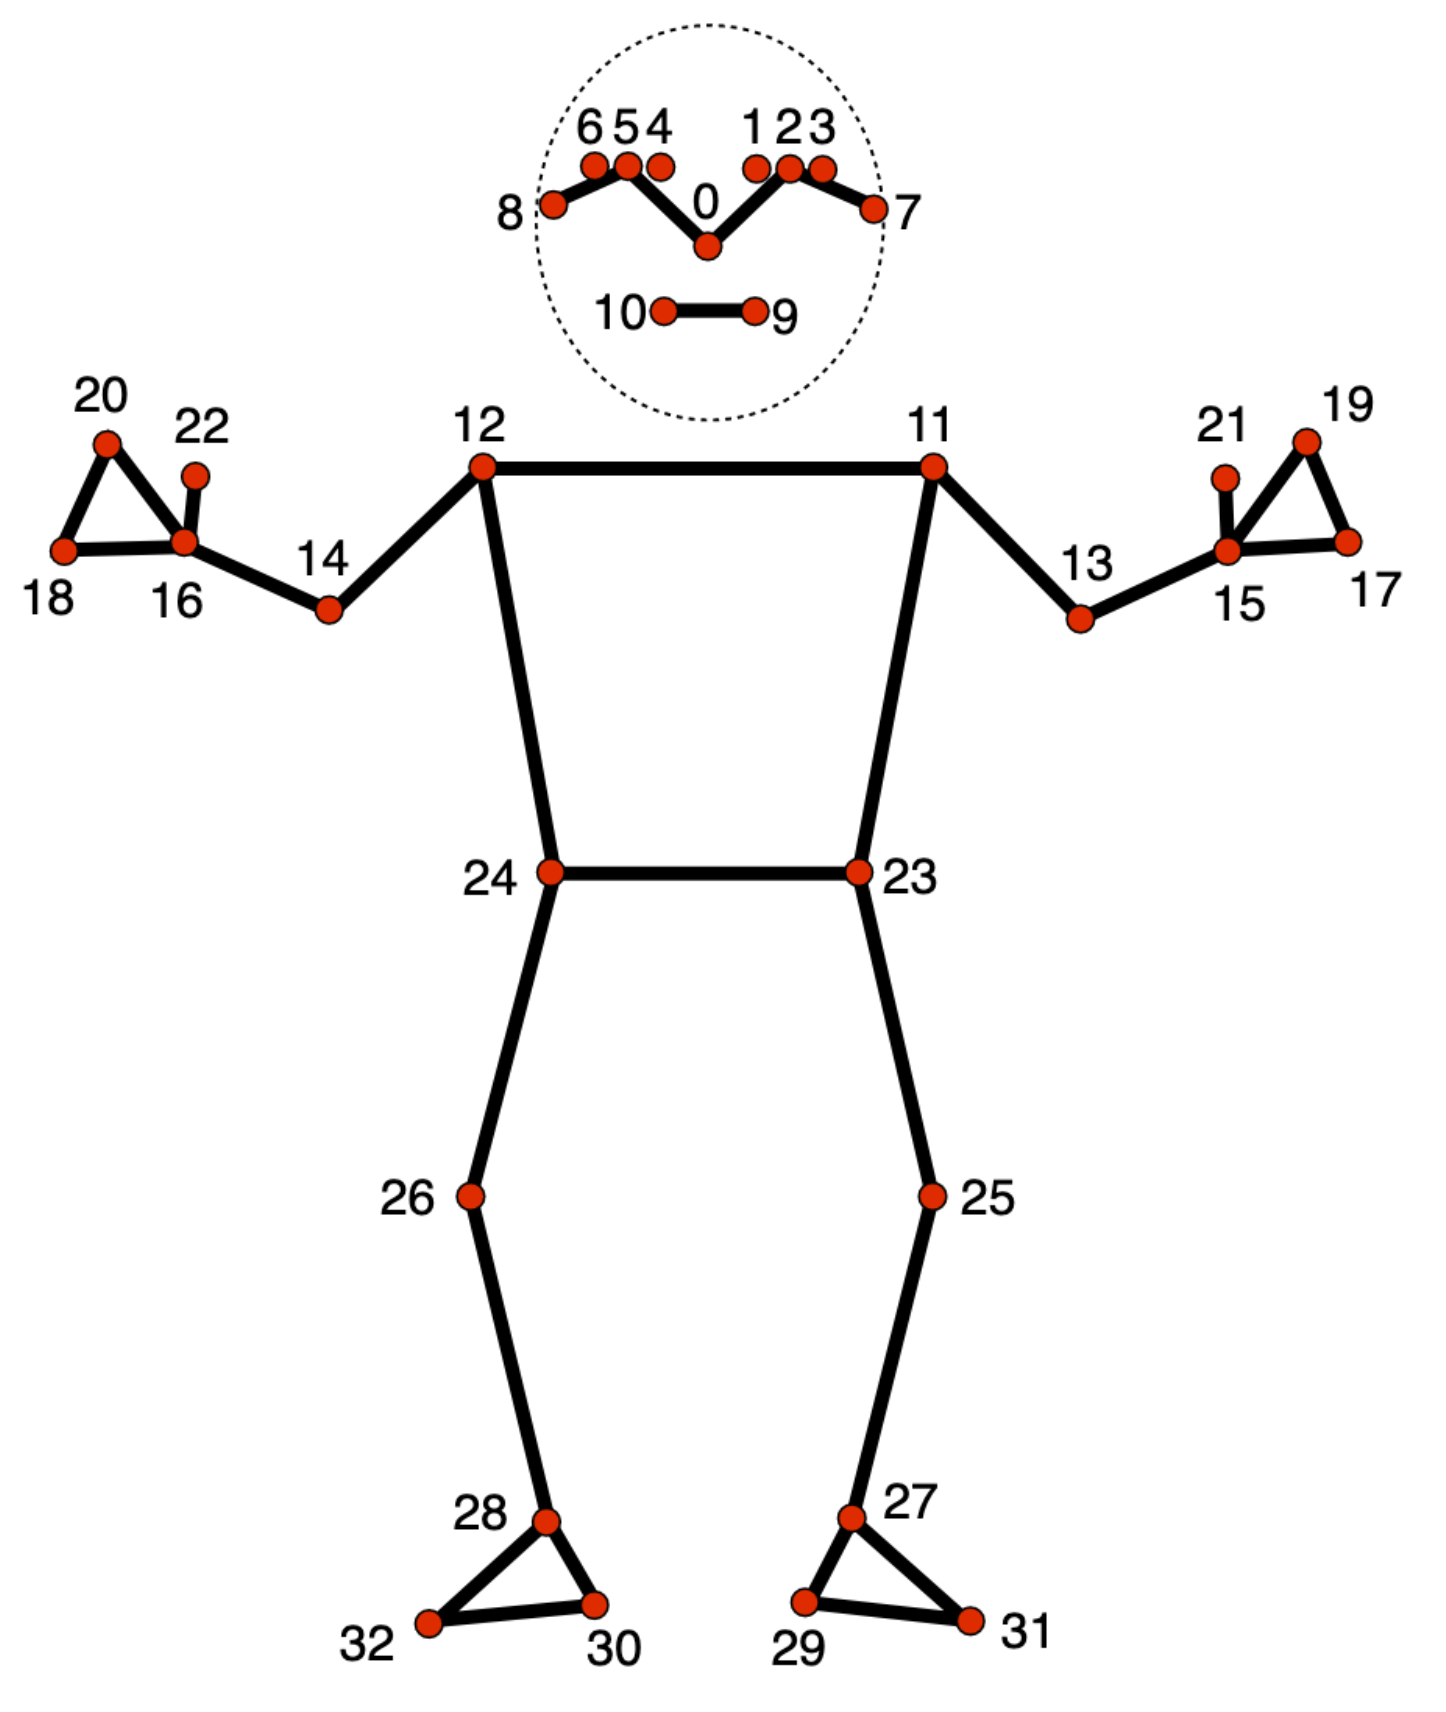
\includegraphics[width=0.9\linewidth]{images/pose_landmarks_index.png}
		% \caption{Landmarks for pose estimation model by MediaPipe}
		\label{fig:pose_landmarks}
	\end{minipage}% <-- Add this percentage sign here
	\begin{minipage}{0.48\textwidth}
		\centering
		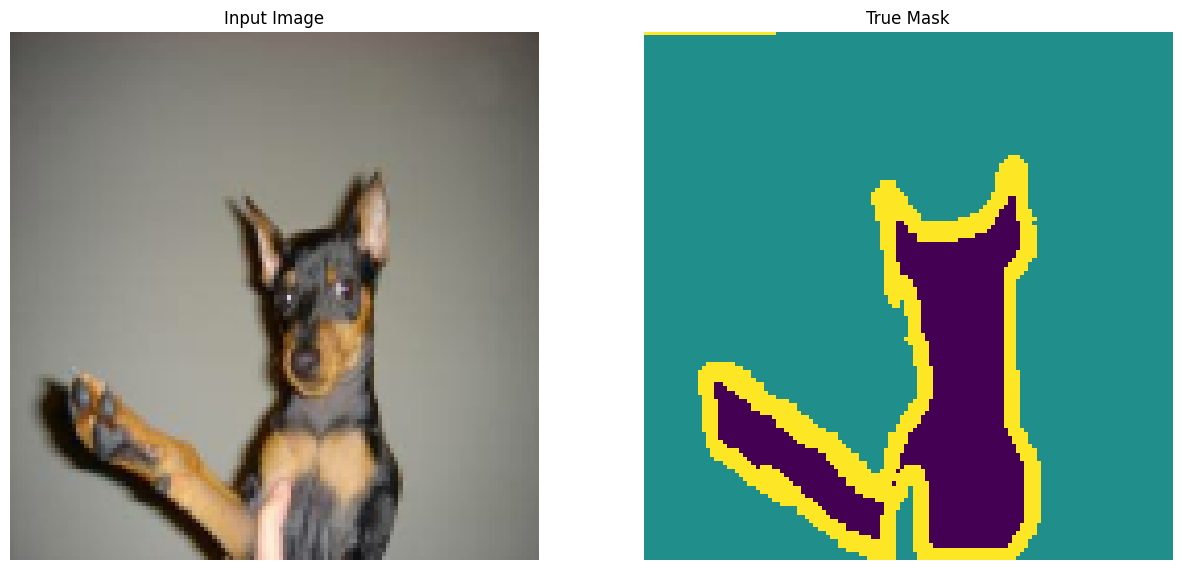
\includegraphics[width=\linewidth]{images/dog.png}
		% \caption{U-Net segmentation on an image from Oxford-IIIT Pet Dataset (Parkhi et al, 2012).}
		\label{fig:dog}
	\end{minipage}
	\caption{Landmarks for pose estimation model by MediaPipe and U-Net segmentation on an image from Oxford-IIIT Pet Dataset (Parkhi et al, 2012).}
	\label{fig:both_figures} % This label can now be used to reference both images together
\end{figure}

\section{Neural Networks}
An artificial intelligence technique called a neural network trains computers to process information like that of the human brain. It uses connected nodes or neurons arranged in a layered pattern to mimic the organization of the human brain. Computers can utilize this adaptive approach to learn from their errors and keep getting better. As a result, artificial neural networks try to more accurately answer challenging problems, such as document summarization and face recognition.
\newline Neural networks consist of neurons in the input layer connected to neurons in the output layer of the network. In Figure \ref{fig:neural_network}, where a general neural network schemes, we can see that they're joined via intermediate neurons. They're placed in hidden layers. 'Hidden' because, in the use of neural networks, only the input and output are of concern to the user. 



\begin{figure}[htp]
	\centering
	\begin{tikzpicture}[
		>=Stealth,
		input/.style={},
		weights/.style={},
		neuron/.style={
			circle,
			draw,
			thick,
			minimum size=1cm,
			fill=white
		},
		function/.style={
			rectangle,
			draw,
			thick,
			minimum size=1cm
		}
		]
		
		% Inputs
		\node[input] (Input-1) at (0,-1) {$x_1$};
		\node[input] (Input-2) at (0,-2) {$x_2$};
		\node[input] (Input-n) at (0,-3) {$x_n$};
		\node at (0,-2.4) {$\vdots$};
		
		% Weights
		\node[weights] (Weights-1) at (2,-1) {$w_1$};
		\node[weights] (Weights-2) at (2,-2) {$w_2$};
		\node[weights] (Weights-n) at (2,-3) {$w_n$};
		
		% Arrows for weights
		\draw[->, thick] (Input-1) -- (Weights-1);
		\draw[->, thick] (Input-2) -- (Weights-2);
		\draw[->, thick] (Input-n) -- (Weights-n);
		
		% Summation circle
		\node[neuron] (Sum) at (4, -2.5) {$\sum$};
		
		% Bias
		\node[input] (Bias) at (4,-4) {$b$};
		
		% Activation function
		\node[function] (Activation) at (6, -2.5) {$f$};
		
		% Output
		\node[input] (Output) at (8, -2.5) {$\hat{y}$};
		
		% Arrows from weights and bias to sum
		\foreach \i in {1,2,n} {
			\draw[->, thick] (Weights-\i.east) -- (Sum.west);
		}
		\draw[->, thick] (Bias) -- (Sum);
		
		% Arrow from the sum to activation function
		\draw[->, thick] (Sum) -- (Activation);
		
		% Arrow from activation function to output
		\draw[->, thick] (Activation) -- (Output);
		
	\end{tikzpicture}
	
	\caption{Schematic representation of a neuron with inputs, weights, a bias, an activation function, and an output.}
	\label{fig:neuron}
\end{figure}


Neurons are basic building components of neural networks. Each neuron takes inputs ($x_1, x_2, ..., x_n$) which are evaluated by weights ($w_1, w_2, ..., w_n$), which are factors that are changed during training. The weight of the connection affects how much input is passed between neurons. We use the weighted sum of all the inputs, adjusted for the weights of the connections between the inputs and the neuron, to determine the output $\hat{y}$ of the neuron. After summing all inputs multiplied by their weight, a bias $b$ is added. Bias is a constant that shifts the activation function left or right (on x-axis). It tells us how high the weighted sum needs to be before the neuron starts getting meaningfully active. A value that goes into the activation function is then the summation function $\epsilon$,
\begin{equation}
	\epsilon = \sum_{i=1}^{n} x_i w_i + b
	\label{eq:weighted_sum}
\end{equation}
where $n$ is is number of inputs.

\subsection*{Activation Functions}
A neural network's activation function is an essential component. A neural network that lacks an activation function is just a straightforward linear regression model. This indicates that the neural network's non-linearity is provided by the activation function. When computing a weighted some like in \ref{eq:weighted_sum}, we can come out with any number. But for most networks, we want its activations (outputs) to be a value between 0 and 1.\newline
There are many types of activation functions, eg. threshold, sigmoid, rectifier, hyperbolic tangent, and softmax. We'll discuss a few of them.

\subsubsection*{Sigmoid Function}
The data science community is familiar with the sigmoid function from its application in logistic regression. Any value can be entered into the sigmoid function, but it will always return a value between 0 and 1. In image classification tasks, the sigmoid function can be used to convert the linear model's output to probability. This probability can be used to predict the binary classification problem (whether there's a cat or a dog in the image). The sigmoid function has the following mathematical definition:

\begin{equation}
	\sigma(z) = \frac{1} {1 + e^{-z}}
\end{equation}

\subsubsection*{SoftMax Function
}
Softmax function is very similar to a sigmoid function. In multiclass classification problems the sigmoid function isn't useful Applying a threshold for positive prediction of 0.5, would say the input data belongs to two classes. The sigmoid function also doesn't take into account the probability of belonging to other classes, when calculating probability for another class. 

Softmax converts numbers or logits (outputs of neural networks) into probabilities. It works with relative probabilities.

Just like with the sigmoid function, in equation \ref{eq:softmax}, an exponential ensures non-linearity; with $z$ values from the neurons of the output layer for $K$ classes. They are then divided by the sum of exponential values to normalize them before being converted to probabilities. The $i$-th entry can be thought of as the predicted probability of the test input belonging to class i.


\begin{equation}
	\sigma(z_i) = \frac{e^{z_{i}}}{\sum_{j=1}^K e^{z_{j}}} \ \ \ \text{for}\ i=1,2,\dots,K
	\label{eq:softmax}
\end{equation}

\begin{figure}[htp]
	\centering
	\begin{tikzpicture}[
		box/.style={
			draw,
			thick,
			rectangle,
			minimum height=1cm,
			minimum width=1.2cm, % Reduced width of boxes
			text width=1.2cm,      % Reduced text width inside boxes
			align=center,
			scale=0.8,           % Scale down everything inside the boxes
		},
		node distance=0.5cm,     % Reduced distance between nodes
		scale=1.2,               % Scale the entire tikzpicture
		every node/.style={transform shape} % This ensures that the scaling affects all nodes
		]
		
		% Define nodes
		\node[box] (image) {image of a bird};
		\node[box, right=of image] (layers) {layers of NN};
		\node[box, right=of layers, text width=1.5cm] (logits) {2.5\\1.3\\0.2\\4.6};
		\node[box, right=of logits] (softmax) {softmax function};
		\node[box, right=of softmax, text width=1.5cm] (probabilities) {0.75\\0.19\\0.02\\0.04};
		\node[box, right=of probabilities, text width=1.5cm] (classes) {Bird\\Mouse\\Cat\\Worm};
		
		% Connect nodes
		\draw[-stealth] (image) -- (layers);
		\draw[-stealth] (layers) -- (logits);
		\draw[-stealth] (logits) -- (softmax);
		\draw[-stealth] (softmax) -- (probabilities);
		\draw[-stealth] (probabilities) -- (classes);
		
		% Add titles above boxes
		\node[above=1mm of logits] {Logits};
		\node[above=1mm of probabilities] {Probabilities};
		\node[above=1mm of classes] {Classes};
		
	\end{tikzpicture}
	\caption{A diagram of the NN softmax classification process.}
\end{figure}

\subsubsection*{Rectifier 
	Function}
Unlike the sigmoid function, the rectifier function does not have the same smoothness property. It is still highly used in the deep learning community. The definition of the rectifier function outputs 0 if the input value is less than 0. The function outputs the input if it isn't. It helps to maintain mathematical stability and keep learned values from being stuck around 0 or jumping into infinity.


\begin{equation}
	Relu(x) = max(0, x)
\end{equation}

Rectified Linear Unit activation function, or ReLU for short, is a common term for rectifier function.\newline
While the softmax function works with the output of the last layer of the neural network, the ReLu function is activated in hidden layers.
\begin{figure}[h]
	\centering
	\begin{minipage}{.5\textwidth}
		\centering
		\begin{tikzpicture}
			\begin{axis}[
				width=\linewidth, % Ensures the plot occupies the full width of the minipage
				height=5cm, % Explicit height
				axis lines=middle,
				xmax=10,
				xmin=-10,
				ymin=-0.05,
				ymax=1.05,
				xlabel={$x$},
				ylabel={$y$}
				]
				\addplot [domain=-9.5:9.5, samples=100,
				thick, blue] {1/(1+exp(-x))};
			\end{axis}
		\end{tikzpicture}
	\end{minipage}%
	\begin{minipage}{.5\textwidth}
		\centering
		\begin{tikzpicture}
			\begin{axis}[
				width=\linewidth, % Ensures the plot occupies the full width of the minipage
				height=5cm, % Explicit height
				axis lines=middle,
				xmax=6,
				xmin=-6,
				ymin=-0.05,
				ymax=5.05,
				xlabel={$x$},
				ylabel={$y$},
				xtick={-6, -3, 0, 3, 6},
				ytick={0, 1, 2, 3, 4, 5}
				]
				\addplot [domain=-5.5:5.5, samples=100, thick, blue] {max(0, x)};
			\end{axis}
		\end{tikzpicture}
		
	\end{minipage}
	\caption{Softmax/Sigmoid function and Rectifier function.}
	\label{fig:foftmaxrelu}
\end{figure}

After applying application function $f$, the output of the neuron would then be: 

\begin{equation}
	\hat{y} = f (\epsilon) = f (\sum_{i=1}^{n} x_i w_i + b)
	\label{eq:forpass}
\end{equation}

If we're discussing a neuron in the hidden or output layers, the equation can be rewritten as:

\begin{equation}
	a_i^k =f\left(\sum_{i=1}^{n} w_{ij}^k a_j^{k-1} + b_i^k\right)
	\label{eq:forpasshidden}
\end{equation}

This output is often called an activation $a$. It represents the sum of all neurons in the ($k-1$) layer. The weight $w^k$ is defined for each layer, $k$. The entries of the weights $w^k$ are just the weights connecting to the $k$-th layer of neurons, that is, the entry in the $i$-th row and $j$-th column is $w^k_{ij}$.


\section{Learning}

During training, a function is passed from one neuron to another, either through a function \ref{eq:forpass} for hidden and output layers or through a weighted sum function \ref{eq:weighted_sum} for the input layer. This is known as the forward pass. When the end of the network is reached, the feed-forward is also completed.\newline
The used dataset is commonly split into a training set, on which the model trains, and a validation set, that evaluates the output of the model. 
As the true results are known during the training phase, the error can be calculated by comparing the actual and predicted values. Cost functions are used to obtain an error value.\newline
%cost functions
There are many loss functions used, based on the nature of the problem. A few of them are: mean squared error, used for regression tasks, binary cross entropy, and categorical cross entropy.
\subsubsection*{Cost functions}
As we train the model, we’ll want to evaluate its accuracy using a cost (or loss) function. The cost function tells us about how well our algorithm models our dataset. The loss error is calculated for each training sample, while the loss function represents the whole set of $m$ samples. The cost function represents the average loss error for a sample. It is a function that assesses how well an ML model performs with a given set of data. The error between expected and predicted values is quantified by the cost function and shown as a single real number. Cost functions can be formed in a variety of ways, depending on the nature of the problem.
\paragraph{Mean squared error}\mbox{}\\
For a model using a formula \ref{eq:forpasshidden},
the commonly used loss function used for regression tasks, is the mean squared error (MSE). 
The cost for a single training example x may be written as


\begin{equation}
	MSE = \frac{1}{2m} \sum_{i=1}^{m} (y_i - a_i)^2,
\end{equation}
where
$i$ represents the index of the sample,
$a$ is the predicted outcome,
$y$ is the actual value, and
$m$ is the number of samples.

\paragraph{Crossentropy function}\mbox{}\\
Other names for cross-entropy loss include logistic loss, log loss, and logarithmic loss. Every predicted class probability is compared to the actual class probability, and a loss function is used to penalize the probability according to its deviation from the actual expected value. Because the penalty is logarithmic, large differences near 1 will result in a large score, and small differences approaching 0 will result in a small score. Cross-entropy loss in a perfect model is 0.
What is meant by cross-entropy is:
\begin{equation}
	-\sum_{c=1}^My_{o,c}\log(p_{o,c}),
\end{equation}
where $M$ is number of classes, $y$ is the binary indicator if class of label $c$ is the correct classification for observation $o$ and $p$ is the predicted probability.

When dealing with labels that are one-hot encoded, such as the 3-class classification problem, where the values are [1,0,0], [0,1,0], and [0,0,1], categorical cross-entropy is employed.
Labels in sparse categorical cross-entropy are encoded with integers, such as [1], [2], and [3] for a 3-class problem.



There are many other types of cost functions used in ML, e.g. Root Mean Square error (RMSE), Binary Cross Entropy Loss Function,  Categorical cross-entropy, Hinge Loss, Kullback-Liebler Divergence LOSS (KL-Divergence), and Huber Loss. Choosing a cost function will be influenced by the type of problem, the output activation function, and the network architecture.


%koniec cost functions
With multi-class, single-label classification problems, as we'll deal with, the first choices of activation and loss functions are ReLU for hidden layers, softmax for the last layer, and categorical crossentropy as a loss function.



The training of a neural network begins with the random assignment of weights and biases (usually to 0) between the nodes. After the initial forward pass, the output layer is highly variable and lacks an identifiable pattern. To address this, a cost function is used to determine the error between the output and the desired values. 

The goal is to enable the computer to find appropriate settings for all of the parameters - weights and biases. That also means minimizing the cost function. \newline
In ML, minimizing the cost (loss) function is done by optimizers. Common optimizers include gradient descent, stochastic gradient descent, or Adam optimizer.


\textbf{Gradient Descent} is a fundamental optimization algorithm used in classification problems and linear regression. It calculates the first derivatives of the cost function to find the minimum. 
Each negative gradient component provides two pieces of information. The sign indicates whether the corresponding input vector component should be increased or decreased. Importantly, the relative magnitudes of all the components indicate which changes are more significant for the cost function output.
However, Gradient Descent may sometimes be trapped in a local minimum and unable to determine the global minimum.\\
\textbf{Stochastic gradient} descent algorithms are a variant of the gradient descent method used in ML. In stochastic gradient descent, instead of computing the gradient using all the observations, only a small random sample of the training data is used to estimate the gradient. This method can significantly reduce the computation time, making it a useful approach in many machine learning applications.\\
\textbf{Adam} is convenient for most convex optimization problems with large datasets. It combines adaptive methods and momentum methods, where it takes into account the moving average of the gradient's first and second-order moments. This allows it to effectively adapt the learning rates for each parameter.
It is an extension of stochastic gradient descent.\newline
Minimizing the cost functions means a better performance on all samples. The algorithm for computing the gradient efficiently is called the backpropagation.
\subsubsection*{Backpropagation}
The backpropagation algorithm is the foundation of neural network learning. The goal of backpropagation is to understand how altering the weights and biases in a network alters the cost function. \newline
In backpropagation, the partial derivatives $\partial C / \partial w^k_{ij}$ and $\partial C / \partial b^k_i$ are computed, calling $C$ the cost. \newline
Let's say we work with a cost function (MSE) for one training example in a simple network, such as in Figure \ref{fig:backprop}: $C_0 (w_1, w_2, \dots, w_{n}) = (a^k - y)^2$.\newline
\begin{figure}
	\centering
	\begin{tikzpicture}[node distance=1.5cm, auto]
		% Define nodes
		\node (a) {\( a^{(k-1)} \)};
		\node[below of=a] (w) {\( w^{(k)} \)};
		\node[right of=w] (z) {\( \epsilon^k \)};
		\node[right of=z] (aL) {\( a^{(k)} \)};
		\node[below of=w] (b) {\( b^k\)};
		\node[right of=aL] (C) {\( \color{red} C_0 \)};
		\node[below of=C] (y) {\( y \)};
		
		% Draw arrows
		\draw[->] (a) -- (z);
		\draw[->] (w) -- (z);
		\draw[->] (z) -- (aL);
		\draw[->] (aL) -- (C);
		\draw[->] (b) -- (z);
		\draw[->] (y) -- (C);
	\end{tikzpicture}
	\caption{An example structure for backpropagation.}
	\label{fig:backprop}
\end{figure}
We want to find the effect of the weight change on the cost function. In ML, the chain rule is often considered in the context of networks.
The last activation $a^k$ is determined by the weighted sum $\epsilon^k$, or a weight $w^k$ multiplied by the previous neuron's activation $a^{(k-1)}$ plus some bias $b^k$. After an activation function, $a^k = f(\epsilon^k)$. These parameters, along with a constant $y$ (wanted output), let us compute the cost.\newline
If the question is how sensitive the cost function is to small changes in our weight $w^k$, we simply calculate the derivative of $C_0$ with respect to $w^k$, using the chain rule.
The equation is as follows:
\begin{equation} 
	\frac{\partial C_0 }{\partial w^k} = 
	{\color{magenta}\frac{\partial \epsilon^k }{\partial w^k}} 
	{\color{violet}\frac{\partial a^k }{\partial \epsilon^k}} 
	{\color{blue}\frac{\partial C_0 }{\partial a^k}} 
\end{equation}
With the computed derivatives:
\begin{equation}
	\frac{\partial C_0}{\partial w^k} =
	{\color{magenta}a^{(k-1)}}
	{\color{violet}f'(\epsilon^k)}
	{\color{blue}2(a^k - y)}
\end{equation}
It's worth noting that the last derivative multiplies the difference between the network's output and the thing we want it to be, so if that output is very different, even slight changes stand to have a big impact on the final cost.\newline
This was computed only for a single training example. Since the full cost function involves averaging together all the cost across many different training examples, its derivative requires averaging the expression over all $n$ training examples:
\begin{equation*}
	\frac{\partial C}{\partial w^{k}} = \frac{1}{n} \sum_{i=0}^{n-1} \frac{\partial C_i}{\partial w^{k}}
\end{equation*}
Of course, that is just one component $w^k$ (in layer $k$) of the gradient vector $\nabla C$, which itself is built up from partial derivatives of the cost function with respect to all the weights and biases.
The sensitivity to bias is almost identical:
\begin{equation*}
	\frac{\partial C_0}{\partial b^{k}} = \frac{\partial \epsilon^{k}}{\partial b^{k}} \frac{\partial a^{k}}{\partial \epsilon^{k}} \frac{\partial C_0}{\partial a^{k}} = 1 \cdot f'(\epsilon^{k}) \cdot 2(a^{k} - y)
\end{equation*}
We want to see how sensitive this cost function is to the activation of the previous layer. The derivative of the weighted sum $\epsilon$ with respect to the activation in the previous layer, comes out to be the the weight.

\begin{equation*}
	\frac{\partial C_0}{\partial a^{(k-1)}} = \frac{\partial \epsilon^{k}}{\partial a^{(k-1)}} \frac{\partial a^{k}}{\partial z^{k}} \frac{\partial C_0}{\partial a^{k}} = w^{k} f'(\epsilon^{k}) 2(a^{k} - y)
\end{equation*}


When $\partial C / \partial \epsilon_i^k$ is close to 0, we can say that the neuron is already near optimal.
Let's call $C$ a cost function for an average weight or a bias, and $-\nabla C$ a negative gradient of the cost function. 
\begin{equation}
	-\nabla C(w_1, w_2, \dots, w_{n}) = 
	\begin{bmatrix}
		-0.08 \\
		+0.12 \\
		-1.06 \\
		\vdots \\
		+0.04
	\end{bmatrix}
	\label{eq:nabla}
\end{equation}

In equation \ref{eq:nabla}, the negative gradients for each weight (their average), are already calculated. So for the cost function to get closer to a minimum, the weights need to be changed accordingly. The cost function is sensitive to the weight $w_1$ of $0.08$. 
After this is computed the weight just needs to be updated in the way:
\begin{equation*}
	w_1= w_1 -\alpha \frac{\partial C}{\partial w_1} ,
\end{equation*}

Where $\alpha$ is a learning rate, which determines the gradient’s influence, and $\frac{\partial C}{\partial w_1} $ is the partial derivative of the cost function $C$ with respect to $w_1$.\newline
In summary, the training can be divided into a few steps:
\begin{enumerate}[label=\arabic*.]
	\item Forward Pass til the final predictions are made.
	\item Loss Calculation
	\item Backward Pass (Backpropagation)
	\item Weight Update
\end{enumerate}
This entire process is repeated for a specified number of epochs or until another stopping criterion is met (like the early stopping callback, which halts training if the validation loss doesn't improve for a set number of epochs).
\begin{figure}[htp]
	\centering
	\begin{tikzpicture}[
		plain/.style={
			draw=none,
			fill=none,
		},
		dot/.style={draw,shape=circle,minimum size=3pt,inner sep=0,fill=black
		},
		net/.style={
			matrix of nodes,
			nodes={
				draw,
				circle,
				inner sep=8.5pt
			},
			nodes in empty cells,
			column sep=0.6cm,
			row sep=-11pt
		},
		>=latex
		]
		\matrix[net] (mat)
		{
			|[plain]| \parbox{1cm}{\centering Input\\layer}
			& |[plain]| \parbox{1cm}{\centering Hidden\\layer}
			& |[plain]| \parbox{1cm}{\centering Output\\layer} \\
			& |[plain]|                 \\
			|[plain]| &            & |[plain]|    \\
			& |[plain]|  &              \\
			|[plain]| & |[dot]|                   \\
			& |[plain]|  & |[dot]|      \\
			|[plain]| & |[dot]|    & |[plain]|    \\
			|[dot]|   & |[plain]|  & |[dot]|      \\
			|[dot]|   & |[dot]|    & |[plain]|    \\
			|[dot]|   & |[plain]|  &              \\
			|[plain]| &            & |[plain]|    \\
			& |[plain]|                 \\
		};
		\foreach \ai/\mi in {2/I1,4/I2,6/I3,12/In}
		\draw[<-] (mat-\ai-1) -- node[above] {\mi} +(-1cm,0);
		\foreach \ai in {2,4,6,12}
		{\foreach \aii/\mii in {3/H1,11/Hm}
			\draw[->] (mat-\ai-1) -- (mat-\aii-2) node[yshift=0.6cm] {\mii};
		}
		\foreach \ai in {3,11}
		{  \draw[->] (mat-\ai-2) -- (mat-4-3);
			\draw[->] (mat-4-3) -- node[above] {O1} +(1cm,0);}
		\foreach \ai in {3,11}
		{  \draw[->] (mat-\ai-2) -- (mat-10-3);
			\draw[->] (mat-10-3) -- node[above] {Op} +(1cm,0);}
	\end{tikzpicture}
	
	\caption{Structure of neural network}
	\label{neural_n_example}
\end{figure}
\subsection*{Hyperparameters of Neural Networks}
\begin{itemize}
	\item Learning Rate is a crucial parameter that controls to which extent the model needs to be modified. It determines the step size at each training iteration. It is usually a value between 0 and 1. We can determine the direction of a loss function's optimum by computing the loss function's gradient. The step size in that direction is determined by the learning rate parameter.
	\item Batch size tells us how much data is changed during 1 cycle (one epoch) of training. The data is subdivided into batches and each step is computed with respect to a batch. Larger batch sizes could lead to faster training but with a trade-off for lower accuracy or overfitting \cite{DBLP:journals/corr/abs-2006-08517}. The best size will depend on several variables, such as the size of the training dataset, the complexity of the model, and the available computational resources.
	\item Epochs define the number of times that the learning algorithm will work through the entire training dataset. Every sample in the training dataset has had a chance to update the internal model parameters after one epoch. One or more batches make up an epoch.
\end{itemize}
\subsubsection*{Regulations of Neural Network}
When talking about the regulation of neural networks we can mention techniques like dropout or early stopping.\newline
Dropout is a regularization strategy for neural networks that, with a given probability, drops a unit (along with connections) during training. It randomly sets a fraction of inputs to 0 at each update during training.
The goal is to stop co-adaptation, which occurs when a neural network becomes overly dependent on a single connection and may be an indication of overfitting. It makes intuitive sense to think of dropout as the formation of an implicit neural network ensemble. The result of dropout is shown in Figure \ref{fig:dropout}
\def\layersep{2}
\def\nodesep{1.5}
\begin{figure}[htp]
	\centering
	\begin{tikzpicture}[
		node/.style={circle, draw, thick},
		scale=0.7, % Adjust the scaling factor as needed
		transform shape,
		every node/.style={scale=0.8} % Adjust the node text scaling factor as needed
		]
		
		\foreach \y in {1,...,5}{
			\node[node] (i\y) at (0,\nodesep*\y) {};
			\node[node, right=\layersep of i\y] (h1\y) {};
			\node[node, right=\layersep of h1\y] (h2\y) {};
		}
		
		\node[node, right=\layersep of h22] (o1) {};
		\node[node, right=\layersep of h24] (o2) {};
		
		\foreach \source in {1,...,5}
		\foreach \dest in {1,...,5}{
			\path[-stealth, thick] (i\source) edge (h1\dest);
			\path[-stealth, thick] (h1\source) edge (h2\dest);
		}
		\foreach \source in {1,...,5}
		\foreach \dest in {1,2}
		\draw[-stealth, thick] (h2\source) -- (o\dest);
		
		\draw[-stealth, thick] (7.5,3*\nodesep) -- node[above,font=\Large] {dropout} (9.5, 3*\nodesep);
		
		% Boundary
		
		\foreach \y in {1,...,5}
		\node[node, right=15em of h2\y] (di\y) {};
		
		\node[red,font=\huge] at (di1) {$\times$};
		\node[red,font=\huge] at (di3) {$\times$};
		
		\foreach \y in {1,...,5}
		\node[node, right=\layersep of di\y] (dh1\y) {};
		
		\node[red,font=\huge] at (dh11) {$\times$};
		\node[red,font=\huge] at (dh13) {$\times$};
		\node[red,font=\huge] at (dh14) {$\times$};
		
		\foreach \y in {1,...,5}
		\node[node, right=\layersep of dh1\y] (dh2\y) {};
		
		\node[red,font=\huge] at (dh22) {$\times$};
		\node[red,font=\huge] at (dh24) {$\times$};
		
		\node[node, right=\layersep of dh22] (do1) {};
		\node[node, right=\layersep of dh24] (do2) {};
		
		\foreach \source in {2,4,5}
		\foreach \dest in {2,5}
		\draw[-stealth, thick] (di\source) -- (dh1\dest);
		
		\foreach \source in {2,5}
		\foreach \dest in {1,3,5}
		\draw[-stealth, thick] (dh1\source) -- (dh2\dest);
		
		\foreach \source in {1,3,5}
		\foreach \dest in {1,2}
		\draw[-stealth, thick] (dh2\source) -- (do\dest);
		
	\end{tikzpicture}
	\caption{Visualization of dropout.}
	\label{fig:dropout}
\end{figure}
\newline An intuitive technique for training just enough is early stopping. It prevents the model from learning on a 'noised' dataset. When training, after every epoch, the model is evaluated using a validation dataset. The training process is terminated if the model's performance on the validation dataset begins to drop (for example, if loss starts to rise or accuracy starts to fall).





%types of models
%neural networks

%use and so on, how works
%rgb gbr conversion

%\section{Types of classifiers and models for Computer Vision}
%An algorithm, or the set of rules that robots employ to classify data, is called a classifier. %However, the final result of the classifier's machine learning is a classification model. The %data is first classified by the model, which was trained using the classifier.






%\subsection{Input Image Processing}
%color, background, extracting landmarks for mediapipe model no. 2, with vs without Mediapipe




\iffalse
/*\section{Gesture Recognition}

Gesture recognition is the practice of identifying hand gestures as input, and translating them into a meaningful command for devices. Dynamic gestures involve a series of changing poses, whereas static gestures remain fixed. Our focus is on recognizing static gestures via a vision-based approach. Vision-based gesture recognition technology is a growing field of study, researchers have developed various methods for feature extraction, including geometric features, moment features, contour features, histograms of oriented gradients, and wavelet features. Examples include a geometric descriptor based on lines connecting the hand contour\cite{lopez2019gesture}, a method based on hand shape \cite{article}, masked Zernike moment features \cite{park2014hand}, geometry-based normalizations \cite{priyal2013robust}, edge orientation histograms. Other techniques include saliency-based features, sparse representation, and geometric features. The recognition algorithm used in these studies includes a weighted AdaBoost classifier based on finger-earth mover's distance and SVM models. Deep learning-based neural networks have shown potential in recognizing hand gestures, using methods like segmented binary images, restricted Boltzmann Machines, pose-guided ensemble networks, and hybrid feature attention networks. However, these methods are not robust enough to handle the complexity of hand gesture images in unconstrained environments.


\fi


